%!TEX root = forallxyyc.tex
\part{Interpretations}
\label{ch.semantics}
\addtocontents{toc}{\protect\mbox{}\protect\hrulefill\par}


\chapter{Extensionality}\label{s:Interpretations}

Recall that TFL is a truth-functional language. Its connectives are all truth-functional, and \emph{all} that we can do with TFL is key sentences to particular truth values. We can do this \emph{directly}. For example, we might stipulate that the TFL sentence `$P$' is to be true. Alternatively, we can do this \emph{indirectly}, offering a symbolization key, e.g.:
	\begin{ekey}
		\item[P] Big Ben is in London.
	\end{ekey}
 But recall from \S\ref{s:TruthFunctionality} that this is \emph{just} a means of specifying `$P$'s truth value; the symbolization key statement amounts to something like the following stipulation: 
	\begin{ebullet}
		\item The TFL sentence `$P$' is true iff Big Ben is in London.
	\end{ebullet}
And we emphasized in \S\ref{s:TruthFunctionality} that TFL cannot handle differences in meaning that go beyond mere differences in truth value.

\section{Symbolizing versus translating}

FOL has some similar limitations. It gets beyond mere truth values, since it enables us to split up sentences into terms, predicates and quantifiers. This enables us to consider what is \emph{true of} some particular object, or of some or all objects. \emph{But that's it}.

To unpack this a bit, consider this symbolization key: 
	\begin{ekey}
		\item[\atom{C}{x}] \gap{x} teaches Logic III in Calgary
	\end{ekey} 
This stipulation does not carry the \emph{meaning} of the English predicate across into our FOL predicate. We are simply stipulating something like this:
	\begin{ebullet}
		\item `$\atom{C}{x}$' and `\gap{x} teaches Logic III in Calgary' are to be \emph{true of} exactly the same things.
	\end{ebullet}
So, in particular:
	\begin{ebullet}
		\item `$\atom{C}{x}$' is to be true of exactly those things which teach Logic III in Calgary (whatever those things might be).
	\end{ebullet}
This is an indirect way of stipulating which things a predicate is true of.

Alternatively, we can stipulate predicate extensions directly. For example, we can stipulate that `$\atom{C}{x}$' is to be true of Richard Zach, and Richard Zach alone. As it happens, this direct stipulation would have the same effect as the indirect stipulation, since Richard, and Richard alone, teaches Logic~III in Calgary. Note, however, that the English predicates `\blank\ is Richard Zach' and `\blank\ teaches Logic III in Calgary' have very different meanings!

The point is that FOL has no resources for dealing with nuances of meaning. When we interpret FOL, all we are considering is what the predicates are true of, regardless of whether we specify these things directly or indirectly. The things a predicate is true of are known as the \define{extension} of that predicate. We say that FOL is an \define{extensional language} because FOL does not represent differences of meaning between predicates that have the same extension.    

This is why we speak of \emph{symbolizing} English sentences in FOL. It is doubtful that we are \emph{translating} English into FOL, for translation should preserve meaning.

\section{Extensions}\label{sec:extensions}
We can stipulate directly what predicates are to be true of. And our stipulations can be as arbitrary as we like. For example, we could stipulate that `$\atom{H}{x}$' should be true of, and only of, the following objects:
	\begin{center}
		Justin Trudeau\\
		the number $\pi$\\
		every top-F key on every piano ever made
	\end{center}
Armed with this interpretation of `$\atom{H}{x}$', suppose we now add to our symbolization key:
	\begin{ekey}
		\item[j] Justin Trudeau
		\item[a] Angela Merkel
		\item[p] the number $\pi$
	\end{ekey}
Then `$\atom{H}{j}$' and `$\atom{H}{p}$' will both be true, on this interpretation, but `$\atom{H}{a}$' will be false, since Angela Merkel was not among the stipulated objects.

This process of explicit stipulation is sometimes described as stipulating the \emph{extension} of a predicate. Note that, in the stipulation we just gave, the objects we listed have nothing particularly in common. This doesn't matter. Logic doesn't care about what we humans (at a particular moment) think `naturally goes together'; to logic, all objects are on an equal footing.

Any well-defined collection of objects is a potential extension of a one-place predicate.  The example above shows one way of stipulating the extension of `$\atom{H}{x}$' by \emph{enumeration}, i.e., we simply list the objects in the extension of~`$\atom{H}{x}$'. We can also stipulate the extension, as we have also already seen, by giving an English predicate, such as `\gap{x} teaches Logic~III at Calgary' or `\gap{x} is an even integer between $3$ and $9$'. The latter would specify an extension consisting of, and only of, $4$, $6$, and~$8$.

Note that some predicates of English, such as `\gap{x} is a round square', are not true of anything.  In this case we say the extension of the predicate is \emph{empty}.  We do allow empty extensions, and we can stipulate that the extension of `$\atom{H}{x}$' is to be empty simply by not listing any members. (It may be odd to consider collections of no things, but logic is odd this way sometimes.)


\section{Many-place predicates}
All of this is quite easy to understand when it comes to one-place predicates, but it gets messier when we deal with two-place predicates. Consider a symbolization key like:
	\begin{ekey}
		\item[\atom{L}{x,y}] \gap{x} loves \gap{y}
	\end{ekey}
Given what we said above, this symbolization key should be read as saying:
	\begin{earg}
		\item[\textbullet] `$\atom{L}{x,y}$' and `\gap{x} loves \gap{y}' are to be true of exactly the same things.
	\end{earg}
So, in particular:
	\begin{earg}
		\item[\textbullet] `$\atom{L}{x,y}$' is to be true of x and y (in that order) iff x loves y.
	\end{earg}
It is important that we insist upon the order here, since love---famously---is not always reciprocated. (Note that `x' and `y' on the right here are symbols of augmented English, and that they are being \emph{used}. By contrast, `$x$' and `$y$' in `$\atom{L}{x,y}$' are symbols of FOL, and they are being \emph{mentioned}.)

That is an indirect stipulation. What about a direct stipulation? This is also tricky. If we \emph{simply} list objects that fall under `$\atom{L}{x,y}$', we will not know whether they are the lover or the beloved (or both). We have to find a way to include the order in our explicit stipulation.

To do this, we can specify that two-place predicates are true of \emph{pairs} of objects, where the order of the pair is important. Thus we might stipulate that `$\atom{B}{x,y}$' is to be true of, and only of, the following pairs of objects:
	\begin{center}
		\ntuple{Lenin, Marx}\\
		\ntuple{de Beauvoir, Sartre}\\
		\ntuple{Sartre, de Beauvoir}
	\end{center}
Here the angle-brackets keep us informed concerning order. Suppose we now add the following stipulations:
	\begin{ekey}
		\item[l] Lenin
		\item[m] Marx
		\item[b] de Beauvoir
		\item[r] Sartre
	\end{ekey}
Then `$\atom{B}{l,m}$' will be true, since \ntuple{Lenin, Marx} is in our explicit list, but `$\atom{B}{m,l}$' will be false, since \ntuple{Marx, Lenin} is not in our list. However, both `$\atom{B}{b,r}$' and `$\atom{B}{r,b}$' will be true, since both \ntuple{de Beauvoir, Sartre} and \ntuple{Sartre, de Beauvoir} are in our explicit list.

To make these ideas more precise, we would need to develop some very elementary \emph{set theory}. Set theory has formal apparatus which allows us to deal with extensions, ordered pairs, and so forth. However, set theory is not covered in this book. So I shall leave these ideas at an imprecise level. Nevertheless, the general idea should be clear.


\section{Semantics for identity}
Identity is a special predicate of FOL. We write it a bit differently than other two-place predicates: `$x=y$' instead of `$\atom{I}{x,y}$' (for example). More important, though, is that its interpretation is fixed, once and for all.

If two names refer to the same object, then swapping one name for another will not change the truth value of any sentence. So, in particular, if `$a$' and `$b$' name the same object, then all of the following will be true:\label{model.nonidentity}
	\begin{align*}
	 	\atom{A}{a} &\eiff \atom{A}{b} \\
	 	\atom{B}{a} &\eiff \atom{B}{b}\\
		\atom{R}{a,a} &\eiff \atom{R}{b,b}\\
		\atom{R}{a,a} & \eiff \atom{R}{a,b}\\
		\atom{R}{c,a} &\eiff \atom{R}{c,b}\\
		\forall x\, \atom{R}{x,a} &\eiff \forall x\, \atom{R}{x,b}
	\end{align*}
Some philosophers have believed the reverse of this claim. That is, they have believed that when exactly the same sentences (not containing `$=$') are true of $a$ and $b$, then $a$ and $b$ are the very same object. This is a highly controversial philosophical claim---sometimes called the \emph{identity of indiscernibles}---and our logic will not subscribe to it; we allow that exactly the same things might be true of two \emph{distinct} objects.  

To bring this out, consider the following interpretation:
	\begin{ebullet}
		\item[\text{domain}:] P.~D.\ Magnus, Tim Button
		\item[$a$:] P.~D.\ Magnus
		\item[$b$:] Tim Button
		\item For every primitive predicate we care to consider, that predicate is true of \emph{nothing}.
	\end{ebullet}
Suppose `$A$' is a one-place predicate; then `$\atom{A}{a}$' is false and `$\atom{A}{b}$' is false, so `$\atom{A}{a} \eiff \atom{A}{b}$' is true. Similarly, if `$R$' is a two-place predicate, then `$\atom{R}{a,a}$' is false and `$\atom{R}{a,b}$' is false, so that `$\atom{R}{a,a} \eiff \atom{R}{a,b}$' is true. And so it goes: every atomic sentence not involving `$=$' is false, so every biconditional linking such sentences is true. For all that, Tim Button and P.~D.\ Magnus are two distinct people, not one and the same!

\section{Interpretations}
We defined a \define{valuation} in TFL as any assignment of truth and falsity to sentence letters. In FOL, we are going to define an \define{interpretation} as consisting of four things:
	\begin{ebullet}
		\item the specification of a domain
		\item for each sentence letter we care to consider, a truth value
		\item for each name that we care to consider, an assignment of exactly one object within the domain
		\item for each predicate that we care to consider (apart from
		`$=$'), a specification of what things (in what order) the
		predicate is to be true of.
	\end{ebullet}
We don't need to specify anything for`$=$', since it has a
\emph{fixed} meaning, namely that of identity. Everything is identical
to itself, and only to itself. 

The symbolization keys that we considered in Part~\ref{ch.FOL} consequently give us one very convenient way to present an interpretation. We will continue to use them in this chapter. Following the discussion of \S\ref{sec:extensions}, we now also allow extensions specified by enumerations on the right side, e.g.,
\begin{ekey}
	\item[\text{domain}] heads of state, numbers
	\item[\atom{H}{x}] Justin Trudeau, Angela Merkel, $\pi$
\end{ekey}
is a perfectly good way of specifying an interpretation, as is
\begin{ekey}
	\item[\text{domain}] $0$, $1$, $2$
	\item[\atom{L}{x,y}] \ntuple{$0$,$1$}, \ntuple{$0$, $2$}, \ntuple{$1$, $2$}
\end{ekey}
We could have specified the same extension (on this particular domain) by giving the English predicate `\gap{x} is less than \gap{y}'.


\newglossaryentry{interpretation}{
  name = {interpretation},
  description = {A specification of a \gls{domain} together with the objects the \glspl{name} pick out and which objects the \glspl{predicate} are true of}
}

However, it is sometimes also convenient to present an interpretation \emph{diagrammatically}. To illustrate (literally): suppose we want to consider just a single two-place predicate, `$\atom{R}{x,y}$'. Then we can represent it just by drawing an arrow between two objects, and stipulate that `$\atom{R}{x,y}$' is to hold of $x$ and $y$ just in case there is an arrow running from $x$ to $y$ in our diagram. As an example, we might offer:
\begin{center}
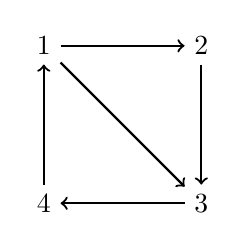
\begin{tikzpicture}
\node (atom1) at (0,2) {$1$};
\node (atom2) at (2,2) {$2$};
\node (atom3) at (2,0) {$3$};
\node (atom4) at (0,0) {$4$};
\draw[->, thick] (atom1)--(atom2);
\draw[->, thick] (atom2)--(atom3);
\draw[->, thick] (atom3)--(atom4);
\draw[->, thick] (atom4)--(atom1);
\draw[->, thick] (atom1) -- (atom3);
\end{tikzpicture}
\end{center}
This diagram could be used to describe an interpretation whose domain is the first four positive whole numbers, and which interprets `$\atom{R}{x,y}$' as being true of and only of:
	\begin{center}
		\ntuple{$1$, $2$}, 
		\ntuple{$2$, $3$}, 
		\ntuple{$3$, $4$}, 
		\ntuple{$4$, $1$}, 
		\ntuple{$1$, $3$}
	\end{center}
Equally we might offer this diagram:

\begin{center}
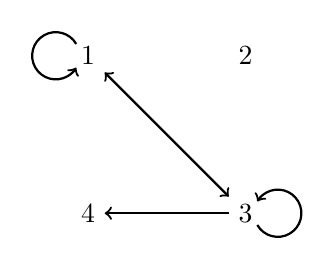
\begin{tikzpicture}
\node (atom1) at (0,2) {$1$};
\node (atom2) at (2,2) {$2$};
\node (atom3) at (2,0) {$3$};
\node (atom4) at (0,0) {$4$};
\draw[->, thick] (atom3)--(atom4);
\draw[->, thick] (atom1)+(-0.15,0.15) arc (-330:-30:.3); 
\draw[->, thick] (atom3)+(0.15,-0.15) arc (-150:150:.3); 
\draw[<->, thick] (atom1) -- (atom3);
\end{tikzpicture}
\end{center}

The interpretation specified by this diagram can also be given by listing what's in the domain and in the extension of~`$\atom{R}{x,y}$':
	\begin{ekey}
	\item[\text{domain}] $1$, $2$, $3$, $4$
	\item[R(x,y)] \ntuple{$1$, $3$}, 
		\ntuple{$3$, $1$}, 
		\ntuple{$3$, $4$}, 
		\ntuple{$1$, $1$},
		\ntuple{$3$, $3$}
	\end{ekey}
If we wanted, we could make our diagrams more complex. For example, we could add names as labels for particular objects. Equally, to symbolize the extension of a one-place predicate, we might simply draw a circle around some particular objects and stipulate that the thus encircled objects (and only them) are to fall under the predicate `$\atom{H}{x}$', say. To specify multiple predicates we could use colored (or dashed, dotted) lines for arrows and circles.


\chapter{Truth in FOL}\label{s:TruthFOL}
We have introduced you to interpretations. Since, among other things, they tell us which predicates are true of which objects, they will provide us with an account of the truth of atomic sentences. However, we now need to say, precisely, what it is for an arbitrary FOL sentence to be true or false in an interpretation.

We know from \S\ref{s:FOLSentences} that there are three kinds of sentence in FOL: 
	\begin{ebullet}
		\item atomic sentences
		\item sentences whose main logical operator is a sentential connective
		\item sentences whose main logical operator is a quantifier
	\end{ebullet}
We need to explain truth for all three kinds of sentence.

We will provide a completely general explanation in this section. However, to try to keep the explanation comprehensible, we will, at several points, use the following interpretation:
	\begin{ekey}
		\item[\text{domain}] all people born before 2000 \textsc{ce}
		\item[a] Aristotle
		\item[b] Beyonc\'e
		\item[\atom{P}{x}] \gap{x} is a philosopher
		\item[\atom{R}{x,y}] \gap{x} was born before \gap{y}
	\end{ekey}
This will be our \emph{go-to example} in what follows.

\section{Atomic sentences}
The truth of atomic sentences should be fairly straightforward. For sentence letters, the interpretation specifies if they are true or false. The sentence `$\atom{P}{a}$' should be true just in case `$\atom{P}{x}$' is true of `$a$'. Given our go-to interpretation, this is true iff Aristotle is a philosopher. Aristotle is a philosopher. So the sentence is true. Equally, `$\atom{P}{b}$' is false on our go-to interpretation.

Likewise, on this interpretation, `$\atom{R}{a,b}$' is true iff the object named by `$a$' was born before the object named by `$b$'. Well, Aristotle was born before Beyonc\'e. So `$\atom{R}{a,b}$' is true. Equally, `$\atom{R}{a,a}$' is false: Aristotle was not born before Aristotle.

Dealing with atomic sentences, then, is very intuitive. When \metav{R} is an $n$-place predicate and $\metav{a}_1$, $\metav{a}_{2}$, \dots, $\metav{a}_{n}$ are names, 

	\factoidbox{
		The sentence $\atom{\metav{R}}{\metav{a}_{1},\metav{a}_{2},\dots,\metav{a}_{n}}$ is true in an interpretation \textbf{iff}\\
		$\metav{R}$ is true of the objects named by $\metav{a}_{1}$, $\metav{a}_{2}$, \dots, $\metav{a}_{n}$ (in that order) in that interpretation.
	}
Recall, though, that there is a special kind of atomic sentence: two names connected by an identity sign constitute an atomic sentence. This kind of atomic sentence is also easy to handle. Where \metav{a} and \metav{b} are any names, 
	\factoidbox{
		$\metav{a} = \metav{b}$ is true in an interpretation \textbf{iff}\\
		 \metav{a} and \metav{b} name the very same object in that interpretation
	}
So in our go-to interpretation, `$a = b$' is false, since Aristotle is distinct from Beyonc\'e.


\section{Sentential connectives}
We saw in \S\ref{s:FOLSentences} that FOL sentences can be built up from simpler ones using the truth-functional connectives that were familiar from TFL. The rules governing these truth-functional connectives are \emph{exactly} the same as they were when we considered TFL. Here they are:
	\factoidbox{
		$\metav{A} \eand \metav{B}$ is true in an interpretation \textbf{iff}\\ both $\metav{A}$ is true and $\metav{B}$ is true in that interpretation.
		
		\medskip
		
		$\metav{A} \eor \metav{B}$ is true in an interpretation \textbf{iff}\\ either $\metav{A}$ is true or $\metav{B}$ is true in that interpretation.

		\medskip
		$\enot \metav{A}$ is true in an interpretation \textbf{iff} \\$\metav{A}$ is false in that interpretation.

		\medskip
		$\metav{A} \eif \metav{B}$ is true in an interpretation \textbf{iff}\\ either $\metav{A}$ is false or $\metav{B}$ is true in that interpretation.

		\medskip
		$\metav{A} \eiff \metav{B}$ is true in an interpretation \textbf{iff} \\$\metav{A}$ has the same truth value as $\metav{B}$ in that interpretation.
	}
This presents the very same information as the characteristic truth tables for the connectives; it just does so in a slightly different way. Some examples will probably help to illustrate the idea. (Make sure you understand them!) On our go-to interpretation:
	\begin{earg}
		\item[\textbullet] `$a = a \eand \atom{P}{a}$' is true
		\item[\textbullet] `$\atom{R}{a,b} \eand \atom{P}{b}$' is false because, although `$\atom{R}{a,b}$' is true, `$\atom{P}{b}$' is false
		\item[\textbullet] `$a = b \eor \atom{P}{a}$' is true
		\item[\textbullet] `$\enot a = b$' is true
		\item[\textbullet] `$\atom{P}{a} \eand \enot( a= b \eand \atom{R}{a,b})$' is true, because `$\atom{P}{a}$' is true and `$a = b$' is false
	\end{earg}
Make sure you understand these examples.

\section[Quantifiers]{When the main logical operator is a quantifier}\label{s:MainLogicalOperatorQuantifier}
The exciting innovation in FOL, though, is the use of \emph{quantifiers}, but expressing the truth conditions for quantified sentences is a bit more fiddly than one might first expect.

Here is a na\"{i}ve first thought. We want to say that `$\forall x\, \atom{F}{x}$' is true iff `$\atom{F}{x}$' is true of everything in the domain. This should not be too problematic: our interpretation will specify directly what `$\atom{F}{x}$' is true of.

Unfortunately, this na\"{i}ve thought is not general enough. For example, we want to be able to say that `$\forall x \exists y\, \atom{L}{x,y}$' is true just in case (speaking roughly) `$\exists y\, \atom{L}{x,y}$' is true of everything in the domain. But our interpretation does not \emph{directly} specify what `$\exists y\, \atom{L}{x,y}$' is true of. Instead, whether or not this is true of something should follow just from the interpretation of the predicate `$L$', the domain, and the meanings of the quantifiers.

So here is a second na\"{i}ve thought. We might try to say that `$\forall x \exists y\, \atom{L}{x,y}$' is to be true in an interpretation iff $\exists y\, \atom{L}{\metav{a},y}$ is true for \emph{every} name \metav{a} that we have included in our interpretation. Similarly, we might try to say that $\exists y\, \atom{L}{\metav{a},y}$ is true just in case $\atom{L}{\metav{a},\metav{b}}$ is true for \emph{some} name \metav{b} that we have included in our interpretation.

Unfortunately, this is not right either. To see this, observe that our go-to interpretation only interprets \emph{two} names, `$a$' and `$b$'. But the domain---all people born before the year 2000 \textsc{ce}---contains many more than two people. (And we have no intention of trying to correct for this by naming \emph{all} of them!)

So here is a third thought. (And this thought is not na\"{i}ve, but correct.) Although it is not the case that we have named \emph{everyone}, each person \emph{could} have been given a name. So we should focus on this possibility of extending an interpretation by adding a new name. We will offer a few examples of how this might work, centering on our go-to interpretation, and we will then present the formal definition.

In our go-to interpretation, `$\exists x\, \atom{R}{b,x}$' should be true. After all, in the domain, there is certainly someone who was born after Beyonc\'e. Lady Gaga is one of those people. Indeed, if we were to extend our go-to interpretation---temporarily, mind---by adding the name `$c$' to refer to Lady Gaga, then `$\atom{R}{b,c}$' would be true on this extended interpretation. This, surely, should suffice to make `$\exists x\, \atom{R}{b,x}$' true on the original go-to interpretation.

In our go-to interpretation, `$\exists x (\atom{P}{x} \eand \atom{R}{x,a})$' should also be true. After all, in the domain, there is certainly someone who was both a philosopher and born before Aristotle. Socrates is one such person. Indeed, if we were to extend our go-to interpretation by letting a new name, `$c$', denote Socrates, then `$\atom{P}{c} \eand \atom{R}{c,a}$' would be true on this extended interpretation. Again, this should surely suffice to make `$\exists x (\atom{P}{x} \eand \atom{R}{x,a})$' true on the original go-to interpretation.

In our go-to interpretation, `$\forall x \exists y\, \atom{R}{x,y}$' should be false. After all, consider the last person born in the year 1999. We don't know who that was, but if we were to extend our go-to interpretation by letting a new name, `$d$', denote that person, then we would not be able to find anyone else in the domain to denote with some further new name, perhaps `$e$', in such a way that `$\atom{R}{d,e}$' would be true. Indeed, no matter \emph{whom} we named with `$e$', `$\atom{R}{d,e}$' would be false. This observation is surely sufficient to make `$\exists y\, \atom{R}{d,y}$' \emph{false} in our extended interpretation, which in turn is surely sufficient to make `$\forall x \exists y\, \atom{R}{x,y}$' false on the original go-to interpretation.

If you have understood these three examples, that's what matters. It provides the basis for a formal definition of truth for quantified sentences.

Strictly speaking, though, we still need to \emph{give} that definition. The result, sadly, is a bit ugly, and requires a few new definitions. Brace yourself!

Suppose that \metav{A} is a formula containing at least one occurrence of the variable \metav{x}, and that $\metav{x}$ is free in $\metav{A}$. We will write this thus:
$$\metav{A}(\ldots \metav{x} \ldots \metav{x} \ldots)$$
Suppose also that \metav{c} is a name. Then we will write:
$$\metav{A}(\ldots \metav{c} \ldots \metav{c} \ldots)$$
for the formula we obtain by replacing \emph{every} occurrence of $\metav{x}$ in \metav{A} with~$\metav{c}$. The resulting formula is called a \define{substitution instance} of $\forall \metav{x}\metav{A}$ and $\exists\metav{x}\metav{A}$.  Also, $\metav{c}$ is called the \define{instantiating name}. So:
	$$\exists x (\atom{R}{e,x} \eiff \atom{F}{x})$$
is a substitution instance of 
	$$\forall y \exists x (\atom{R}{y,x} \eiff \atom{F}{x})$$
with the instantiating name `$e$' and instantiated variable~`$y$'.

\newglossaryentry{substitution instance}{
  name = substitution instance,
  description = {The result of replacing every free occurrence of a \gls{variable} in a \gls{formula} with a \gls{name}}
}

Our interpretation will include a specification of which names correspond to which objects in the domain. Take any object in the domain, say, $d$, and a name $\metav{c}$ which is not already assigned by the interpretation. If our interpretation is $\mathbf{I}$, then we can consider the interpretation $\mathbf{I}[d/\metav{c}]$ which is just like $\mathbf{I}$ except it \emph{also} assigns the name $\metav{c}$ to the object~$d$. Then we can say that $d$ \define{satisfies} the formula $\metav{A}(\dots\metav{x}\dots\metav{x}\dots)$ in the interpretation~$\mathbf{I}$ if, and only if, $\metav{A}(\dots\metav{c}\dots\metav{c}\dots)$ is true in $\mathbf{I}[d/\metav{c}]$. (If $d$ satisfies $\metav{A}(\dots\metav{x}\dots\metav{x}\dots)$ we also say that $\metav{A}(\dots\metav{x}\dots\metav{x}\dots)$ is \emph{true of}~$d$.) 

\factoidbox{The interpretation $\mathbf{I}[d/\metav{c}]$ is just like the interpretation $\mathbf{I}$ except it also assigns the name $\metav{c}$ to the object~$d$.

\
\\
An object $d$ \define{satisfies} $\metav{A}(\dots\metav{x}\dots\metav{x}\dots)$ in interpretation~$\mathbf{I}$ \textbf{iff} $\metav{A}(\dots\metav{c}\dots\metav{c}\dots)$ is true in $\mathbf{I}[d/\metav{c}]$.
}

So, for instance, Socrates satisfies the formula~$\atom{P}{x}$ since $\atom{P}{c}$ is true in the interpretation $\mathbf{I}[\text{Socrates}/c]$, i.e., the interpretation:
\begin{ekey}
	\item[\text{domain}] all people born before 2000 \textsc{ce}
	\item[a] Aristotle
	\item[b] Beyonc\'e
	\item[c] Socrates 
	\item[\atom{P}{x}] \gap{x} is a philosopher
	\item[\atom{R}{x,y}] \gap{x} was born before \gap{y}
\end{ekey}

Armed with this notation, the rough idea is as follows. The sentence
$\forall \metav{x}\metav{A}(\ldots \metav{x} \ldots \metav{x} \ldots)$
will be true in $\mathbf{I}$ iff, for any object~$d$ in the domain,
$\metav{A}(\ldots \metav{c} \ldots \metav{c}\ldots)$ is true in
$\mathbf{I}[d/\metav{c}]$, i.e., no matter what object (in the domain)
we name with $\metav{c}$. In other words, $\forall \metav{x}
\metav{A}(\ldots \metav{x} \ldots \metav{x} \ldots)$ is true iff every
object in the domain satisfies $\metav{A}(\ldots \metav{x} \ldots
\metav{x} \ldots)$. Similarly, the sentence $\exists
\metav{x}\metav{A}$ will be true iff there is \emph{some} object that
satisifes $\metav{A}(\ldots \metav{x} \ldots \metav{x} \ldots)$, i.e.,
$\metav{A}(\ldots \metav{c} \ldots \metav{c} \ldots)$ is true in
$\mathbf{I}[d/\metav{c}]$ for some object~$d$.
	\factoidbox{
		$\forall \metav{x}\metav{A}(\ldots \metav{x}\ldots\metav{x}\ldots)$ is true in an interpretation \textbf{iff}\\ 
		every object in the domain satisfies $\metav{A}(\ldots
		\metav{x} \ldots \metav{x}\ldots)$.
		\bigskip
		
		$\exists \metav{x}\metav{A}(\ldots \metav{x}\ldots\metav{x}\ldots)$ is true in an interpretation \textbf{iff}\\ at least one object in the domain satisfies
		$\metav{A}(\ldots \metav{x}\ldots\metav{x}\ldots)$.
	}
To be clear: all this is doing is formalizing (very pedantically) the intuitive idea expressed on the previous page. The result is a bit ugly, and the final definition might look a bit opaque. Hopefully, though, the \emph{spirit} of the idea is clear.

\section{Satisfaction of formulas}

The concept of an object satisfying a formula with a free variable can also be extended to formulas with more than one free variable. If we have a formula $\metav{A}(\metav{x},\metav{y})$ with two free variables $\metav{x}$ and $\metav{y}$, then we can say that a pair of objects $\langle a, b\rangle$ satisfies $\metav{A}(\metav{x},\metav{y})$ iff $\metav{A}(\metav{c},\metav{d})$ is true in the interpretation extended by two names $\metav{c}$ and $\metav{d}$, where $\metav{c}$ names~$a$ and $\metav{d}$ names~$b$. So, for instance, $\langle \text{Socrates}, \text{Plato}\rangle$ satisfies $\atom{R}{x,y}$ since $\atom{R}{c,d}$ is true in the interpretation:
\begin{ekey}
	\item[\text{domain}] all people born before 2000 \textsc{ce}
	\item[a] Aristotle
	\item[b] Beyonc\'e
	\item[c] Socrates
	\item[d] Plato
	\item[\atom{P}{x}] \gap{x} is a philosopher
	\item[\atom{R}{x,y}] \gap{x} was born before \gap{y}
\end{ekey}
For atomic formulas, the objects, pairs of objects, etc., that satisfy them are exactly the extension of the predicate given in the interpretation. But the notion of satisfaction also applies to non-atomic formulas, e.g., the formula $\atom{P}{x} \land \atom{R}{x,b}$ is satisfied by all philosophers born before Beyonc\'e. It even applies to formulas involving quantifiers, e.g., $\atom{P}{x} \eand \lnot\exists y(\atom{P}{y} \land \atom{R}{y,x})$ is satisfied by all people who are philosophers and for whom it is true that no philosopher was born before them---in other words, it is true of the first philosopher.

By considering formulas (possibly involving quantifiers) with two free
variables, we can express relations for which we do not have dedicated
predicate symbols in our interpretation or symbolization key. Consider
the formula $\atom{R}{x,y}$. It expresses the relation `\gap{x} was
born before \gap{y}', since that is how we have specified its
extension. What happens if we switch the variables, i.e., consider
`$\atom{R}{y,x}$'?  A pair of objects \ntuple{$\text{y}, \text{x}$} in
the domain (i.e., a pair of people) satisfies $\atom{R}{y,x}$ if, and only if,
the reverse pair \ntuple{$\text{x}, \text{y}$} satisfies
$\atom{R}{x,y}$. In other words, $\atom{R}{y,x}$ expresses the
relation `\gap{x} was born \emph{after} \gap{y}'. Or suppose we add to
our interpretation a predicate for `teacher of'.
\begin{ekey}
	\item[\atom{T}{x,y}] \gap{x} was a teacher of \gap{y}
\end{ekey}
Then the formula `$\exists z(\atom{T}{z,x} \land \atom{T}{z,y})$' is
satisfied by x and~y if, and only if, some person z was a teacher of
both x and~y, i.e., it expresses `\gap{x} and \gap{y} have a teacher
in common'. Similarly, `$\forall z(\atom{T}{x,z} \eiff \atom{T}{y,
z})$' expresses `\gap{x} and \gap{y} taught the same people'.

\practiceproblems
\solutions
\problempart
\label{pr.TorF1}
Consider the following interpretation:
	\begin{ebullet}
		\item The domain comprises only Corwin and Benedict
		\item `$\atom{A}{x}$' is to be true of both Corwin and Benedict
		\item `$\atom{B}{x}$' is to be true of Benedict only
		\item `$\atom{N}{x}$' is to be true of no one
		\item `$c$' is to refer to Corwin
	\end{ebullet}
Determine whether each of the following sentences is true or false in that interpretation:
\begin{earg}
\item $\atom{B}{c} $
\item $\atom{A}{c}  \eiff \enot \atom{N}{c}$
\item $\atom{N}{c}  \eif (\atom{A}{c} \eor \atom{B}{c})$
\item $\forall x\, \atom{A}{x}$
\item $\forall x \enot \atom{B}{x}$
\item $\exists x(\atom{A}{x} \eand \atom{B}{x})$
\item $\exists x(\atom{A}{x} \eif \atom{N}{x})$
\item $\forall x(\atom{N}{x} \eor \enot \atom{N}{x})$
\item $\exists x\, \atom{B}{x} \eif \forall x\, \atom{A}{x}$
\end{earg}

\problempart
\label{pr.TorF2}
Consider the following interpretation:	
	\begin{ebullet}
		\item The domain comprises only Lemmy, Courtney and Eddy
		\item `$\atom{G}{x}$' is to be true of Lemmy, Courtney and Eddy.
		\item `$\atom{H}{x}$' is to be true of and only of Courtney
		\item `$\atom{M}{x}$' is to be true of and only of Lemmy and Eddy
		\item `$c$' is to refer to Courtney
		\item `$e$' is to refer to Eddy
	\end{ebullet}
Determine whether each of the following sentences is true or false in that interpretation:
\begin{earg}
\item $\atom{H}{c} $
\item $\atom{H}{e} $
\item $\atom{M}{c}  \eor \atom{M}{e}$
\item $\atom{G}{c}  \eor \enot \atom{G}{c}$
\item $\atom{M}{c}  \eif \atom{G}{c}$
\item $\exists x\, \atom{H}{x}$
\item $\forall x\, \atom{H}{x}$
\item $\exists x\, \enot \atom{M}{x}$
\item $\exists x(\atom{H}{x} \eand \atom{G}{x})$
\item $\exists x(\atom{M}{x} \eand \atom{G}{x})$
\item $\forall x(\atom{H}{x} \eor \atom{M}{x})$
\item $\exists x\, \atom{H}{x} \eand \exists x\, \atom{M}{x}$
\item $\forall x(\atom{H}{x} \eiff \enot \atom{M}{x})$
\item $\exists x\, \atom{G}{x} \eand \exists x \enot \atom{G}{x}$
\item $\forall x\exists y(\atom{G}{x} \eand \atom{H}{y})$
\end{earg}

\problempart
\label{pr.TorF3}
Following the diagram conventions introduced at the end of \S\ref{s:Interpretations}, consider the following interpretation:	
\begin{center}
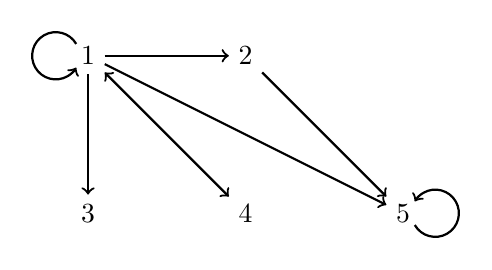
\begin{tikzpicture}
\node (atom1) at (0,2) {$1$};
\node (atom2) at (2,2) {$2$};
\node (atom4) at (0,0) {$3$};
\node (atom5) at (2,0) {$4$};
\node (atom6) at (4,0) {$5$};
\draw[->, thick] (atom1)+(-0.15,0.15) arc (-330:-30:.3); 
\draw[->, thick] (atom6)+(0.15,-0.15) arc (-150:150:.3); 
\draw[->, thick] (atom1) -- (atom2);
\draw[->, thick] (atom1) -- (atom4);
\draw[<->, thick] (atom1) -- (atom5);
\draw[->, thick] (atom1) -- (atom6);
\draw[->, thick] (atom2) -- (atom6);
\end{tikzpicture}
\end{center}
Determine whether each of the following sentences is true or false in that interpretation:
\begin{earg}
\item $\exists x\, \atom{R}{x,x}$
\item $\forall x\, \atom{R}{x,x}$
\item $\exists x \forall y\, \atom{R}{x,y}$
\item $\exists x \forall y\, \atom{R}{y,x}$
\item $\forall x \forall y \forall z ((\atom{R}{x,y} \eand \atom{R}{y,z}) \eif \atom{R}{x,z})$
\item $\forall x \forall y \forall z ((\atom{R}{x,y} \eand \atom{R}{x,z}) \eif \atom{R}{y,z})$
\item $\exists x \forall y\, \enot \atom{R}{x,y}$
\item $\forall x(\exists y\, \atom{R}{x,y} \eif \exists y\, \atom{R}{y,x})$
\item $\exists x \exists y (\enot x = y \eand \atom{R}{x,y} \eand \atom{R}{y,x})$
\item $\exists x \forall y(\atom{R}{x,y} \eiff x = y)$
\item $\exists x \forall y(\atom{R}{y,x} \eiff x = y)$
\item $\exists x \exists y(\enot x = y \eand \atom{R}{x,y} \eand \forall z(\atom{R}{z,x} \eiff y = z))$
\end{earg}


\chapter{Semantic concepts}

Defining truth in FOL was quite fiddly. But now that we are done, we can define various other central logical notions. These definitions will look very similar to those for TFL, from \S\ref{s:SemanticConcepts}. However, remember that they concern \emph{interpretations}, rather than valuations.

We will use the symbol `$\entails$' for FOL much as we did for TFL. So:
	$$\metav{A}_1, \metav{A}_2, \ldots, \metav{A}_n \entails\metav{C}$$
means that there is no interpretation in which all of $\metav{A}_1$, $\metav{A}_2$, \dots, $\metav{A}_n$ are true and in which \metav{C} is false. Derivatively,
	$$\entails\metav{A}$$
means that \metav{A} is true in every interpretation.

The other logical notions also have corresponding definitions in FOL:

\begin{itemize}
\item An FOL sentence $\metav{A}$ is a \define{validity} iff $\metav{A}$ is true in every interpretation; i.e.,  $\entails\metav{A}$.
\newglossaryentry{validity}
{
name=validity,
description={A \gls{sentence of FOL} that is true in every \gls{interpretation}}
}

\item $\metav{A}$ is a \define{contradiction} iff $\metav{A}$ is false in every interpretation; i.e., $\entails\enot\metav{A}$.
\newglossaryentry{contradiction of FOL}
{
  name=contradiction (of FOL),
  text=contradiction,
description={A \gls{sentence of FOL} that is false in every \gls{interpretation}}
}
  
\item $\metav{A}_1, \metav{A}_2, \ldots, \metav{A}_n \therefore \metav{C}$ is \define{valid in FOL} iff there is no interpretation in which all of the premises are true and the conclusion is false; i.e., $\metav{A}_1,\metav{A}_2,\ldots, \metav{A}_n \entails\metav{C}$. It is \define{invalid in FOL} otherwise.
\newglossaryentry{valid in FOL}
{
  name=validity of arguments (in FOL),
  text = valid,
description={A property held by arguments; an argument is valid if and only if no \gls{interpretation} makes all premises true and the conclusion false}
}

\item Two FOL sentences \metav{A} and \metav{B} are \define{equivalent} iff they are true in exactly the same interpretations as each other; i.e., both $\metav{A}\entails\metav{B}$ and $\metav{B}\entails\metav{A}$.

\newglossaryentry{equivalent in FOL}
{
  name=equivalence (in FOL),
  text = equivalent,
description={A property held by pairs of \glspl{sentence of FOL} if and only if the sentences have the same truth value in every \gls{interpretation}}
}

\item The FOL sentences $\metav{A}_1$, $\metav{A}_2$, \dots, $\metav{A}_n$ are \define{jointly satisfiable} iff some interpretation makes all of them true. They are \define{jointly unsatisfiable} iff there is no such interpretation.
\newglossaryentry{satisfiable in FOL}
{
  name=satisfiability (in FOL),
  text=jointly satisfiable,
description={A property held by \glspl{sentence of FOL} if and only if some \gls{interpretation} makes all the sentences true}
}
\end{itemize}

\chapter{Using interpretations}
\label{sec.UsingModels}

\section{Validities and contradictions}
Suppose we want to show that `$\exists x\, \atom{A}{x,x} \eif \atom{B}{d}$' is \emph{not} a validity. This requires showing that the sentence is not true in every interpretation; i.e.,\ that it is false in some interpretation. If we can provide just one interpretation in which the sentence is false, then we will have shown that the sentence is not a validity.

In order for `$\exists x\,\atom{A}{x,x} \eif \atom{B}{d}$' to be false, the antecedent (`$\exists x\, \atom{A}{x,x}$') must be true, and the consequent (`$\atom{B}{d}$') must be false. To construct such an interpretation, we start by specifying a domain. Keeping the domain small makes it easier to specify what the predicates will be true of, so we will start with a domain that has just one member. For concreteness, let's say it is \emph{just} the city of Paris.
	\begin{ekey}
		\item[\text{domain}] Paris
	\end{ekey}
The name `$d$' must refer to something in the domain, so we have no option but:
	\begin{ekey}
		\item[d] Paris
	\end{ekey}
Recall that we want `$\exists x\, \atom{A}{x,x}$' to be true, so we want all members of the domain to be paired with themselves in the extension of `$A$'. We can just offer:
	\begin{ekey}
		\item[\atom{A}{x,y}] \gap{x} is identical with \gap{y}
	\end{ekey}
Now `$\atom{A}{d,d}$' is true, so it is surely true that `$\exists x\, \atom{A}{x,x}$'. Next, we want `$\atom{B}{d}$' to be false, so the referent of `$d$' must not be in the extension of `$B$'. We might simply offer:
	\begin{ekey}
		\item[\atom{B}{x}] \gap{x} is in Germany
	\end{ekey}
Now we have an interpretation where `$\exists x\, \atom{A}{x,x}$' is true, but where `$\atom{B}{d}$' is false. So there is an interpretation where `$\exists x\, \atom{A}{x,x} \eif \atom{B}{d}$' is false. So `$\exists x\, \atom{A}{x,x} \eif \atom{B}{d}$' is not a validity.

We can just as easily show that `$\exists x\atom{A}{x,x} \eif \atom{B}{d}$' is not a contradiction. We need only specify an interpretation in which `$\exists x\atom{A}{x,x} \eif \atom{B}{d}$' is true; i.e., an interpretation in which either `$\exists x\, \atom{A}{x,x}$' is false or `$\atom{B}{d}$' is true. Here is one:
	\begin{ekey}
		\item[\text{domain}] Paris
		\item[d] Paris
		\item[\atom{A}{x,y}] \gap{x} is identical with \gap{y}
		\item[\atom{B}{x}] \gap{x} is in France
	\end{ekey}
This shows that there is an interpretation where `$\exists x\atom{A}{x,x} \eif \atom{B}{d}$' is true. So `$\exists x\, \atom{A}{x,x} \eif \atom{B}{d}$' is not a contradiction.
	\factoidbox{
		To show that $\metav{A}$ is not a validity, it suffices to find an interpretation where $\metav{A}$ is false.
		
		To show that $\metav{A}$ is not a contradiction, it suffices to find an interpretation where $\metav{A}$ is true.
	}

\section{Logical equivalence}
Suppose we want to show that `$\forall x\, \atom{S}{x}$' and `$\exists x\, \atom{S}{x}$' are not logically equivalent. We need to construct an interpretation in which the two sentences have different truth values; we want one of them to be true and the other to be false. We start by specifying a domain. Again, we make the domain small so that we can specify extensions easily. In this case, we will need at least two objects. (If we chose a domain with only one member, the two sentences would end up with the same truth value. In order to see why, try constructing some partial interpretations with one-member domains.) For concreteness, let's take:
	\begin{ekey}
		\item[\text{domain}] Ornette Coleman, Miles Davis
	\end{ekey}
We can make `$\exists x\, \atom{S}{x}$' true by including something in the extension of `$S$', and we can make `$\forall x\, \atom{S}{x}$' false by leaving something out of the extension of `$S$'. For concreteness, let's say:
	\begin{ekey}
		\item[\atom{S}{x}] \gap{x} plays saxophone
	\end{ekey}
Now `$\exists x\, \atom{S}{x}$' is true, because `$\atom{S}{x}$' is true of Ornette Coleman. Slightly more precisely, extend our interpretation by allowing `$c$' to name Ornette Coleman.  `$\atom{S}{c}$' is true in this extended interpretation, so `$\exists x\, \atom{S}{x}$' was true in the original interpretation. Similarly, `$\forall x\, \atom{S}{x}$' is false, because `$\atom{S}{x}$' is false of Miles Davis. Slightly more precisely, extend our interpretation by allowing `$d$' to name Miles Davis, and `$\atom{S}{d}$' is false in this extended interpretation, so `$\forall x\, \atom{S}{x}$' was false in the original interpretation. We have provided a counter-interpretation to the claim that `$\forall x\, \atom{S}{x}$' and `$\exists x\, \atom{S}{x}$' are logically equivalent.
	\factoidbox{
		To show that $\metav{A}$ and $\metav{B}$ are not logically equivalent, it suffices to find an interpretation where one is true and the other is false.
	}

\section{Validity, entailment and satisfiability}
To test for validity, entailment, or satisfiability, we typically need to produce interpretations that determine the truth value of several sentences simultaneously.

Consider the following argument in FOL:
$$\exists x(\atom{G}{x} \eif \atom{G}{a}) \therefore \exists x\, \atom{G}{x} \eif \atom{G}{a}$$
To show that this is invalid, we must make the premise true and the conclusion false. The conclusion is a conditional, so to make it false, the antecedent must be true and the consequent must be false. Clearly, our domain must contain two objects. Let's try:
	\begin{ekey}
		\item[\text{domain}] Karl Marx, Ludwig von Mises
		\item[\atom{G}{x}] \gap{x} hated communism
		\item[a] Karl Marx
	\end{ekey}
Given that Marx wrote \emph{The Communist Manifesto}, `$\atom{G}{a}$' is plainly false in this interpretation. But von Mises famously hated communism, so `$\exists x\, \atom{G}{x}$' is true in this interpretation. Hence `$\exists x\, \atom{G}{x} \eif \atom{G}{a}$' is false, as required.

Does this interpretation make the premise true? Yes it does! Note that `$\atom{G}{a} \eif \atom{G}{a}$' is true. (Indeed, it is a validity.) But then certainly `$\exists x (\atom{G}{x} \eif \atom{G}{a})$' is true, so the premise is true, and the conclusion is false, in this interpretation. The argument is therefore invalid.

In passing, note that we have also shown that `$\exists x(\atom{G}{x} \eif \atom{G}{a})$' does \emph{not} entail `$\exists x\, \atom{G}{x} \eif \atom{G}{a}$', i.e., that $\exists x (\atom{G}{x} \eif \atom{G}{a}) \nentails \exists x \atom{G}{x} \eif \atom{G}{a}$. Equally, we have shown that the sentences `$\exists x (\atom{G}{x} \eif \atom{G}{a})$' and `$\enot (\exists x\, \atom{G}{x} \eif \atom{G}{a})$' are jointly satisfiable.

Let's consider a second example. Consider:
$$\forall x \exists y\, \atom{L}{x,y} \therefore \exists y \forall x\, \atom{L}{x,y}$$
Again, we want to show that this is invalid. To do this, we must make the premises true and the conclusion false. Here is a suggestion:
\begin{ekey}
	\item[\text{domain}] Canadian citizens currently in a domestic partnership with another Canadian citizen
	\item[\atom{L}{x,y}] \gap{x} is in a domestic partnership with \gap{y}
\end{ekey}
The premise is clearly true on this interpretation. Anyone in the domain is a Canadian citizen in a domestic partnership with some other Canadian citizen. That other citizen will also, then, be in the domain. So for everyone in the domain, there will be someone (else) in the domain with whom they are in a domestic partnership. Hence `$\forall x \exists y\, \atom{L}{x,y}$' is true. However, the conclusion is clearly false, for that would require that there is some single person who is in a domestic partnership with everyone in the domain, and there is no such person, so the argument is invalid. We observe immediately that the sentences `$\forall x \exists y\, \atom{L}{x,y}$' and `$\enot\exists y \forall x\, \atom{L}{x,y}$' are jointly satisfiable and that `$\forall x \exists y\, \atom{L}{x,y}$' does not entail `$\exists y \forall x\, \atom{L}{x,y}$'.

For our third example, we'll mix things up a bit. In \S\ref{s:Interpretations}, we described how we can present some interpretations using diagrams. For example:
\begin{center}
	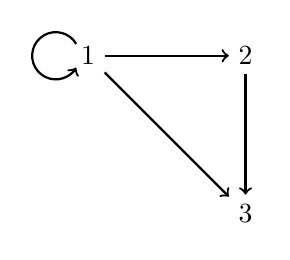
\begin{tikzpicture}
	\node (atom1) at (0,2) {1};
	\node (atom2) at (2,2) {2};
	\node (atom3) at (2,0) {3};
	\draw[->, thick] (atom1)--(atom2);
	\draw[->, thick] (atom1)--(atom3);
	\draw[->, thick] (atom1)+(-0.15,0.15) arc (-330:-30:.3); 
	\draw[->, thick] (atom2) -- (atom3);
	\end{tikzpicture}
\end{center}
Using the conventions employed in \S\ref{s:Interpretations}, the domain of this interpretation is the first three positive whole numbers, and `$\atom{R}{x,y}$' is true of x and y just in case there is an arrow from x to y in our diagram. Here are some sentences that the interpretation makes true:
\begin{ebullet}
	\item `$\forall x \exists y\, \atom{R}{y,x}$' 
	\item `$\exists x \forall y\, \atom{R}{x,y}$' \hfill witness 1
	\item `$\exists x \forall y (\atom{R}{y,x} \eiff x = y)$' \hfill witness 1
	\item `$\exists x \exists y \exists z ((\enot y = z \eand \atom{R}{x,y}) \eand \atom{R}{z,x})$' \hfill witness 2
	\item `$\exists x \forall y\, \enot \atom{R}{x,y}$' \hfill witness 3
	\item `$\exists x (\exists y\, \atom{R}{y,x} \eand \enot \exists y\, \atom{R}{x,y})$' \hfill witness 3
\end{ebullet}
This immediately shows that all of the preceding six sentences are jointly satisfiable. We can use this observation to generate \emph{invalid} arguments, e.g.:
\begin{align*}
	\forall x \exists y\, \atom{R}{y,x}, \exists x \forall y\, \atom{R}{x,y}  &\therefore  \forall x \exists y\, \atom{R}{x,y}\\
	\exists x \forall y\, \atom{R}{x,y}, \exists x \forall y \enot \atom{R}{x,y} & \therefore \enot \exists x \exists y \exists z (\enot y = z \eand (\atom{R}{x,y} \eand \atom{R}{z,x}))
\end{align*}
and many more besides.

\factoidbox{
	If some interpretation makes all of $\metav{A}_1, \metav{A}_2, \ldots, \metav{A}_n$  true and $\metav{C}$ is false, then:
	\begin{ebullet}
		\item$\metav{A}_1, \metav{A}_2, \ldots, \metav{A}_n \therefore \metav{C}$ is \emph{invalid}; and
	\item $\metav{A}_1, \metav{A}_2, \ldots, \metav{A}_n \nentails \metav{C}$; and
	\item 
	And $\metav{A}_1, \metav{A}_2, \ldots, \metav{A}_n, \enot \metav{C}$ are jointly satisfiable.
\end{ebullet}}
An interpretation which refutes a claim---to logical truth, say, or to entailment---is called a \emph{counter-interpretation}, or a \emph{counter-model}.

We'll close this section, though, with a caution about the relationship between (in)validity and (non)entailment. Recall FOL's limitations: it is an extensional language; it ignores issues of vagueness; and it cannot handle cases of validity for `special reasons'. To take one illustration of these issues, consider this natural-language argument: 
\begin{earg}
	\item[] Every fox is cute.
	\item[\therefore] All vixens are cute.
\end{earg}
This is valid: necessarily every vixen is a fox, so it is impossible for the premise to be true and the conclusion false. Now, we might sensibly symbolize the argument as follows:
$$\forall x(\atom{F}{x} \eif \atom{C}{x}) \therefore \forall x(\atom{V}{x} \eif  \atom{C}{x})$$
However, it is easy to find counter-models which show that $\forall x(\atom{F}{x} \eif \atom{C}{x}) \nentails \forall x(\atom{V}{x} \eif  \atom{C}{x})$. (\emph{Exercise}: find one.) So, it would be \emph{wrong} to infer that the English argument is \emph{invalid}, just because there is a counter-model to the relevant \emph{FOL{}-entailment}.

The general moral is this. If you want to infer from the absence of an entailment in FOL to the invalidity of some English argument, then you need to argue that nothing important is lost in the way you have symbolized the English argument.

\practiceproblems

\solutions
\problempart
\label{pr.Contingent}
Show that each of the following is neither a validity nor a contradiction:
\begin{earg}
\item \leftsolutions\ $\atom{D}{a}  \eand \atom{D}{b}$
\item \leftsolutions\ $\exists x\, \atom{T}{x,h}$
\item \leftsolutions\ $\atom{P}{m}  \eand \enot\forall x\, \atom{P}{x}$
\item $\forall z \atom{J}{z} \eiff \exists y\, \atom{J}{y}$
\item $\forall x (\atom{W}{x,m,n} \eor \exists y\atom{L}{x,y})$
\item $\exists x (\atom{G}{x} \eif \forall y\, \atom{M}{y})$
\item $\exists x (x = h \eand x = i)$
\end{earg}

\solutions
\problempart
\label{pr.NotEquiv}
Show that the following pairs of sentences are not logically equivalent.
\begin{earg}
\item $\atom{J}{a} $,  $\atom{K}{a}$
\item $\exists x\, \atom{J}{x}$,  $\atom{J}{m}$
\item $\forall x\, \atom{R}{x,x}$, $\exists x\, \atom{R}{x,x}$
\item $\exists x\, \atom{P}{x} \eif \atom{Q}{c}$, $\exists x (\atom{P}{x} \eif \atom{Q}{c})$
\item $\forall x(\atom{P}{x} \eif \enot \atom{Q}{x})$, $\exists x(\atom{P}{x} \eand \enot \atom{Q}{x})$
\item $\exists x(\atom{P}{x} \eand \atom{Q}{x})$, $\exists x(\atom{P}{x} \eif \atom{Q}{x})$
\item $\forall x(\atom{P}{x}\eif \atom{Q}{x})$, $\forall x(\atom{P}{x} \eand \atom{Q}{x})$
\item $\forall x\exists y\, \atom{R}{x,y}$, $\exists x\forall y\, \atom{R}{x,y}$
\item $\forall x\exists y\, \atom{R}{x,y}$, $\forall x\exists y\, \atom{R}{y,x}$
\end{earg}



\problempart
Show that the following sentences are jointly satisfiable:
\begin{earg}
\item  $\atom{M}{a}, \enot \atom{N}{a}, \atom{P}{a}, \enot \atom{Q}{a}$
\item $\atom{L}{e,e}, \atom{L}{e,g}, \enot \atom{L}{g,e}, \enot \atom{L}{g,g}$
\item $\enot (\atom{M}{a} \eand \exists x\, \atom{A}{x}), \atom{M}{a} \eor \atom{F}{a}, \forall x(\atom{F}{x} \eif \atom{A}{x})$
\item $\atom{M}{a} \eor \atom{M}{b}, \atom{M}{a} \eif \forall x \enot \atom{M}{x}$
\item $\forall y\, \atom{G}{y}, \forall x (\atom{G}{x} \eif \atom{H}{x}), \exists y \enot \atom{I}{y}$
\item $\exists x(\atom{B}{x} \eor \atom{A}{x}), \forall x \enot \atom{C}{x}, \forall x\bigl[(\atom{A}{x} \eand \atom{B}{x}) \eif \atom{C}{x}\bigr]$
\item $\exists x\, \atom{X}{x}, \exists x\, \atom{Y}{x}, \forall x(\atom{X}{x} \eiff \enot \atom{Y}{x})$
\item $\forall x(\atom{P}{x} \eor \atom{Q}{x}), \exists x\enot(\atom{Q}{x} \eand \atom{P}{x})$
\item $\exists z(\atom{N}{z} \eand \atom{O}{z,z}), \forall x\forall y(\atom{O}{x,y} \eif \atom{O}{y,x})$
\item $\enot \exists x \forall y\, \atom{R}{x,y}, \forall x \exists y\, \atom{R}{x,y}$
\item $\enot \atom{R}{a,a}$, $\forall x (x=a \eor \atom{R}{x,a})$
\item $\forall x\forall y\forall z[(x=y \eor y=z )\eor x=z]$, $\exists x\exists y\ \enot x= y$
\item $\exists x\exists y((\atom{Z}{x} \eand \atom{Z}{y} )\eand x=y)$, $\enot \atom{Z}{d}$, $d=e$
\end{earg}

\problempart
Show that the following arguments are invalid:
\begin{earg}
\item $\forall x(\atom{A}{x} \eif \atom{B}{x}) \therefore \exists x\, \atom{B}{x}$
\item $\forall x(\atom{R}{x} \eif \atom{D}{x}), \forall x(\atom{R}{x} \eif \atom{F}{x}) \therefore \exists x(\atom{D}{x} \eand \atom{F}{x})$
\item $\exists x(\atom{P}{x}\eif \atom{Q}{x}) \therefore \exists x\, \atom{P}{x}$
\item $\atom{N}{a} \eand \atom{N}{b} \eand \atom{N}{c} \therefore \forall x\, \atom{N}{x}$
\item $\atom{R}{d,e}, \exists x\, \atom{R}{x,d} \therefore \atom{R}{e,d}$
\item $\exists x(\atom{E}{x} \eand \atom{F}{x}), \exists x\, \atom{F}{x} \eif \exists x\, \atom{G}{x} \therefore \exists x(\atom{E}{x} \eand \atom{G}{x})$
\item $\forall x\, \atom{O}{x,c}, \forall x\, \atom{O}{c,x} \therefore \forall x\, \atom{O}{x,x}$
\item $\exists x(\atom{J}{x} \eand \atom{K}{x}), \exists x \enot \atom{K}{x}, \exists x \enot \atom{J}{x} \therefore \exists x(\enot \atom{J}{x} \eand \enot \atom{K}{x})$
\item $\atom{L}{a,b} \eif \forall x\, \atom{L}{x,b}, \exists x\, \atom{L}{x,b} \therefore \atom{L}{b,b}$
\item $\forall x(\atom{D}{x} \eif \exists y\, \atom{T}{y,x}) \therefore \exists y \exists z\ \enot y= z$
\end{earg}

\chapter{Reasoning about interpretations}

\section{Validities and contradictions}
We can show that a sentence is \emph{not} a validity just by providing one carefully specified interpretation: an interpretation in which the sentence is false. To show that something \emph{is} a validity, on the other hand, it would not be enough to construct ten, one hundred, or even a thousand interpretations in which the sentence is true. A sentence is only a validity if it is true in \emph{every} interpretation, and there are infinitely many interpretations. We need to reason about all of them, and we cannot do this by dealing with them one by one!

Sometimes, we can reason about all interpretations fairly easily. For example, we can offer a relatively simple argument that `$\atom{R}{a,a}\eor\enot \atom{R}{a,a}$' is a validity:
	\begin{quote}
		\label{allmodels1}
		Any relevant interpretation will give `$\atom{R}{a,a}$' a truth value. If `$\atom{R}{a,a}$' is true in an interpretation, then `$\atom{R}{a,a} \eor \enot\atom{R}{a,a}$' is true in that interpretation. If `$\atom{R}{a,a}$' is false in an interpretation, then $\enot\atom{R}{a,a}$ is true, and so `$\atom{R}{a,a} \eor\enot \atom{R}{a,a}$' is true in that interpretation. These are the only alternatives. So `$\atom{R}{a,a} \eor\enot \atom{R}{a,a}$' is true in every interpretation. Therefore, it is a validity.
	\end{quote}
This argument is valid, of course, and its conclusion is true. However, it is not an argument in FOL. Rather, it is an argument in English \emph{about} FOL: it is an argument in the metalanguage.

Note another feature of the argument. Since the sentence in question contained no quantifiers, we did not need to think about how to interpret `$a$' and `$R$'; the point was just that, however we interpreted them, `$\atom{R}{a,a}$' would have some truth value or other. (We could ultimately have given the same argument concerning TFL sentences.)

Let's have another example. The sentence `$\forall x(\atom{R}{x,x}\eor\enot \atom{R}{x,x})$' should obviously be a validity. However, saying \emph{precisely} why is quite tricky. We cannot say that `$\atom{R}{x,x} \eor\enot \atom{R}{x,x}$' is true in every interpretation, since `$\atom{R}{x,x} \eor\enot \atom{R}{x,x}$' is not even a \emph{sentence} of FOL (remember that `$x$' is a variable, not a name). Instead, we should say something like this:
	\begin{quote}
		Consider some arbitrary interpretation. $\forall x(\atom{R}{x,x}\eor \enot\atom{R}{x,x})$ is true in our interpretation iff $\atom{R}{x,x}\eor\enot\atom{R}{x,x}$ is satisfied by every object of its domain. Consider some arbitrary member of the domain, which, for convenience, we will call Fred. Either Fred satisfies $\atom{R}{x,x}$ or it does not. If Fred satisfies `$\atom{R}{x,x}$', then Fred also satisfies `$\atom{R}{x,x} \eor \enot \atom{R}{x,x}$'. If Fred does not satisfy `$\atom{R}{x,x}$', it \emph{does} satisfy `$\enot\atom{R}{x,x}$' and so also `$\atom{R}{x,x} \eor\enot \atom{R}{x,x}$'.\footnote{We use here the fact that the truth conditions for connectives also apply to satisfaction: $a$ satisfies $\metav{A}(\metav{x}) \lor \metav{B}(\metav{x})$ iff $a$ satisfies $\metav{A}(\metav{x})$ or $\metav{B}(\metav{x})$, etc.} So either way, Fred satisfies `$\atom{R}{x,x} \eor\enot \atom{R}{x,x}$'. Since there was nothing special about Fred---we might have chosen any object---we see that every object in the domain satisfies `$\atom{R}{x,x} \eor\enot \atom{R}{x,x}$'. So `$\forall x (\atom{R}{x,x} \eor\enot \atom{R}{x,x})$' is true in our interpretation. But we chose our interpretation arbitrarily, so `$\forall x (\atom{R}{x,x} \eor\enot \atom{R}{x,x})$' is true in every interpretation. It is therefore a validity.
	\end{quote}
This is quite long-winded, but, as things stand, there is no alternative. In order to show that a sentence is a validity, we must reason about \emph{all} interpretations.

\section{Other cases}
Similar points hold of other cases too. Thus, we must reason about all interpretations if we want to show:
	\begin{ebullet}
		\item that a sentence is a contradiction; for this requires that it is false in \emph{every} interpretation.
		\item that two sentences are logically equivalent; for this requires that they have the same truth value in \emph{every} interpretation.
		\item that some sentences are jointly unsatisfiable; for this requires that there is no interpretation in which all of those sentences are true together; i.e., that, in \emph{every} interpretation, at  least one of those sentences is false.
		\item that an argument is valid; for this requires that the conclusion is true in \emph{every} interpretation where the premises are true.
		\item that some sentences entail another sentence.
	\end{ebullet}
The problem is that, with the tools available to you so far, reasoning about all interpretations is a serious challenge! For a final example, here is a perfectly obvious entailment:
	$$\forall x(\atom{H}{x} \eand \atom{J}{x}) \entails \forall x\, \atom{H}{x}$$
After all, if everything is both $H$ and $J$, then everything is~$H$.
But we can only establish the entailment by considering what must be
true in every interpretation in which the premise $\forall
x(\atom{H}{x} \eand \atom{J}{x})$ is true. To show this, we would have
to reason as follows:
	\begin{quote}
		Consider an arbitrary interpretation in which `$\forall x(\atom{H}{x} \eand \atom{J}{x})$' is true. It follows that `$\atom{H}{x} \eand \atom{J}{x}$' is satisfied by every object in this interpretation. `$\atom{H}{x}$' will, then, also be satisfied by every object.\footnote{Here again we make use of the fact that any object that satisfies $\metav{A}(\metav{x}) \land \metav{B}(\metav{x})$ must satisfy both $\metav{A}(\metav{x})$ and $\metav{B}(\metav{x})$.} So it must be that `$\forall x\, \atom{H}{x}$' is true in the  interpretation. We've assumed nothing about the interpretation except that it was one in which `$\forall x(\atom{H}{x} \eand \atom{J}{x})$' is true. So any interpretation in which `$\forall x(\atom{H}{x} \eand \atom{J}{x})$' is true is one in which `$\forall x\, \atom{H}{x}$' is true.
\end{quote}
Even for a simple entailment like this one, the reasoning is somewhat complicated. For more complicated entailments, the reasoning can be extremely torturous.

The following table summarizes whether a single interpretation or counter-interpretation suffices, or whether we must reason about all interpretations.

\begin{center}\small
\begin{tabular}{l l l}
%\cline{2-3}
 & \textbf{Yes} & \textbf{No}\\
 \hline
%\cline{2-3}
validity? & all interpretations & one counter-interpretation\\
contradiction? &  all interpretations  & one counter-interpretation\\
equivalent? & all interpretations & one counter-interpretation\\
satisfiable? & one interpretation & all interpretations\\
valid? & all interpretations & one counter-interpretation\\
entailment? & all interpretations & one counter-interpretation\\
\end{tabular}
\end{center}
\label{table.ModelOrArgument}

You might want to compare this table with the table at the end of \S\ref{s:PartialTruthTable}. The key difference resides in the fact that TFL concerns truth tables, whereas FOL concerns interpretations. This difference is deeply important, since each truth-table only ever has finitely many lines, so that a complete truth table is a relatively tractable object. By contrast, there are infinitely many interpretations for any given sentence(s), so that reasoning about all interpretations can be a deeply tricky business.
